\section{分类相关问题}
\subsection{多分类学习}
考虑用二分类学习器来解决多分类的问题。考虑$N$个类别$C_1,C_2,\cdots,C_N$,则将多分类任务拆分为若干个二分类任务求解,测试时,对这些分类器的预测结果进行集成,以获得最终多分类结果。
\subsubsection{一对一策略(One vs One,OvO)}
对给定数据集$D=\{(\sample{x}{1},\sample{y}{1}),(\sample{x}{2},\sample{y}{2}),\cdots,(\sample{x}{m},\sample{y}{m})\},\sample{y}{i}\in\{ C_1,C_2,\cdots,C_N \}$,OvO将$N$个类别两两配对,产生$\frac{N(N-1)}{2}$个二分类任务,其中,分类器把$D$中的$C_i$类样例作为正例,将$C_j$类样例作为反例。测试时,将新样本提交给所有分类器,得到$\frac{N(N-1)}{2}$个分类结果,最终结果通过投票产生。如下图所示
\begin{center}
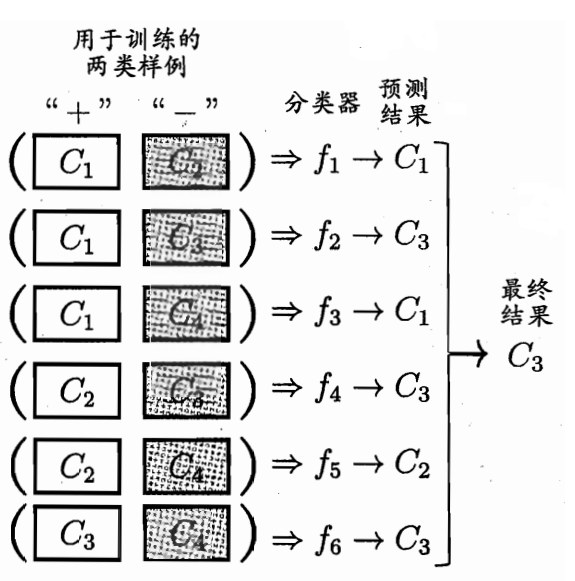
\includegraphics[scale=0.5]{../figures/CP1.PNG} 
\end{center}
可用矩阵来记录这个过程。初始化一个$N\times N$的0矩阵$A$。对于用来训练的两个样例$(C_i,C_j)$,若$C_i$为正例,$C_j$为反例,则记$A_{i,j}=1,A_{j,i}=0$;若$C_i$为反例,$C_j$为正例,则记$A_{i,j}=0,A_{j,i}=1$,如下
\begin{equation}
\begin{pmatrix}
0 & 1 & 0 & 1\\
0 & 0 & 0 & 1\\
1 & 1 & 0 & 1\\
0 & 0 & 0 & 0\\
\end{pmatrix}
\end{equation}
按行求和,可得到$(2,1,3,0)^T$,投票结果为$C_3$最多。则判断为$C_3$。
\subsubsection{一对其余策略(One vs Rest,OvR)}
OvR每次将一个类作为正例,其他类作为反例进行训练,得到$N个$分类器。测试时,若仅有一个分类器预测为正类,则对应的类别标记作为最终的分类结果;若有多个分类器预测为正类,则比较这些分类器的预测置信度,选择置信度最大的。

OvR只需要训练$N$个分类器,而OvO需要训练$\frac{N(N-1)}{2}$个分类器,因而OvO的存储开销和测试时间通常比OvR大,但由于OvO的每个分类器仅用到了两个类的样例,因而OvO的训练时间开销通常比OvR更小。
